\documentclass[12pt,a4paper]{article}
\usepackage{fancyhdr}
\usepackage{fontspec}
\usepackage{amsmath}
\usepackage{amssymb}
\usepackage{bm}
\usepackage{tikz}
\setmainfont{Microsoft YaHei}
\pagestyle{fancy}

\begin{document}

\fancyfoot[C]{by chinasjtu@msn.com }

\newcommand{\nl}{\newline}

\newcommand{\ntinf}{\lim\limits_{n \to \infty}}
\newcommand{\xtinf}{\lim\limits_{x \to \infty}}

\newcommand{\Atinf}{\lim\limits_{A \to \infty}}
\newcommand{\Rtinf}{\lim\limits_{R \to \infty}}

\newcommand{\ntx}[1]{\lim\limits_{n \to #1}}
\newcommand{\xtx}[1]{\lim\limits_{x \to #1}}
\newcommand{\ttx}[1]{\lim\limits_{t \to #1}} 
\newcommand{\ktx}[1]{\lim\limits_{k \to #1}} 
\newcommand{\dxtx}[1]{\lim\limits_{\Delta x \to #1}}

\newcommand{\jfab}{\int_{a}^{b}}
\newcommand{\jf}[2]{\int_{#1}^{#2}}

\newcommand{\nsum}[2]{\sum\limits_{n=#1}^{#2}}
\newcommand{\isum}[2]{\sum\limits_{i=#1}^{#2}}
\newcommand{\ksum}[2]{\sum\limits_{k=#1}^{#2}}

\newcommand{\nsuminf} {\nsum{1}{\infty}}
\newcommand{\ksuminf} {\ksum{1}{\infty}}
\newcommand{\isuminf} {\isum{1}{\infty}}




\begin{center} 第16章 重积分  \end{center}


$记m_i=inf\{f(x,y)\},(x,y)\in \delta_i,M_i=sup\{f(x,y)\},(x,y) \in \delta_i,\omega_i=M_i-m_i$

$s(T)=\Sigma m \Delta \delta_i, S(T)=\Sigma M \Delta \delta_i$

$f在有界闭域D上可积 \Leftrightarrow \dtx{0}(S(T)-s(T))=0$

$有界闭域上连续f必可积$

$\nl$

$定理:若f在有界闭域D上有界,其不连续点只分布在有限条光滑曲线上,则f在D上必可积$

$1^\circ \jf{}{} \jf{}{} d\delta =S$

$2^\circ f(x) \in R[a,b]g(y) \in R[c,d]$

$则f(x)g(y)在D上可积\jf{}{}\jf{}{}fgdxdy=\jf{a}{b}fdx \jf{c}{d}ydy$

$\nl$

$求解\jf{}{}\jf{}{}[x+y]dyxy=6, [0,2]×[0,2]$

$\jf{}{}\jf{}{} \sqrt[3]{1-x^2-y^2} dxdy <0 (x^2+y^2 \le 4)$

$\nl$

$定限原则,将D向x轴投影,得出a \le x \le b,任取x \in [a,b]在D内$

$y积分域,由y_1(x)到y_2(x),再对x由a到b积分(先y后x)$

$\nl$

$改变积分顺序(线到域,域到线)$

$\jf{0}{2a}dx\jf{\sqrt {2ax-x^2}}{\sqrt 2ax}f(x,y)dy(a>0)$

$=\jf{0}{a}dy \jf{\frac{y^2}{2a}}{a-\sqrt{a^2-y^2}}f(x,y)dx+\jf{0}{a}dy\jf{a+\sqrt{a^2-y^2}}{2a}f(x,y)dx+\jf{a}{2a}dy \jf{\frac{y^2}{x}}{2a}f(x,y)dx$

$\nl$

$例:作适当变换,化二重积分\iint_{|x|+|y| \le 1} f(x+y) dxdy 为定积分$

$令u=x-y,v=x+y,则|J|=\frac{1}{2},积分域为D',-1 \le u \le 1$

$-1 \le v \le 1,原式为\jf{-1}{1}f(v)dv$

$\nl$

$Viviand体$

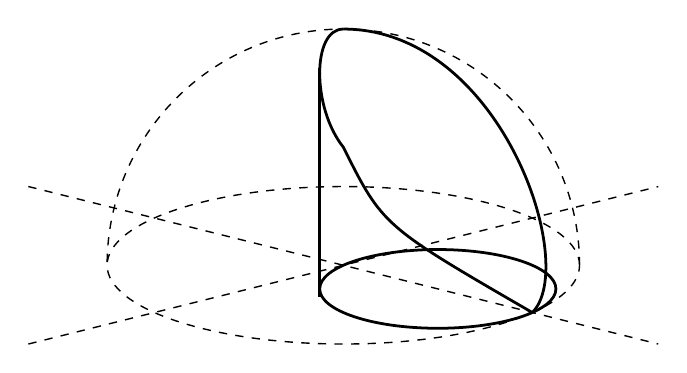
\begin{tikzpicture}[domain=1:5,line width=1pt]
\draw[style=dashed, line width=0.5 pt] (-4,-1) -- (4,1);
\draw[style=dashed, line width=0.5 pt] (-4,1) -- (4,-1);

\draw[style=dashed, line width=0.5 pt]  (0,0)  ellipse  (3 and 1);
\draw[style=dashed, line width=0.5 pt]  (3,0)  arc  (0:180:3);

\draw(2.4,-0.6)..controls (3,0) and (2,3)..(0,3);

\draw  (2.4,-0.6)..controls (0.5,0.5)..(0,1.5)..controls (-0.4,2) and (-0.4,3) .. (0,3);

\draw (1.2,-0.3)  ellipse  (1.5 and 0.5);
\draw (-0.3,-0.4) -- (-0.3,2.5);
\end{tikzpicture}

$\iint_D \sqrt{4-x^2-y^2}dxdy$

$=\jf{}{} \jf{0}{\frac{\pi}{2}}d \theta \jf{0}{acos \theta} \sqrt {a^2-r^2}rdr$

$=\frac{4}{3}a^3(\frac{\pi}{2}-\frac{2}{3})$

$\nl$

$例:求封闭曲线(\frac{x^2}{a^2}+\frac{y^2}{b^2})=x^2-y^2(a,b>0)面积$

$= ab \jf{0}{2\pi}\sqrt{a^2cos^2 \theta -b^2sin^2 \theta}d\theta$

$\nl$

$例:D:x=0,y=0,x+y=0,令u=y-x,v=y+x,则D'=v-u=0,v+u=0,v=2$

$\nl$

$用二重积分证明\jf{a}{b}fdx\jf{a}{b}\frac{1}{f}dx \ge (b-a)^2$

$分析:2 \cdot 原式=\iint_D \frac{f(x)}{f(y)}dxdy+\iint_D \frac{f(y)}{f(x)}dxdy \ge 2 \iint_D dxdy = 2(b-a)^2$

$\nl$

$证明:\frac{\jf{0}{1}xf^2(x)dx}{\jf{0}{1}xf(x)dx} \le \frac{\jf{0}{1}f^2(x)dx}{\jf{0}{1}f(x)dx},f(x)在[0,1]上单调递减,恒正$

$类似上例有I=\frac{1}{2}\iint_D f(x)f(y)(y-x)(f(x)-f(y))dxdy \ge 0$

$\nl$

$证明\iint_D \frac{a\varphi(x)+b\varphi(y)}{\varphi(x)+\varphi(y)}dxdy为常数,\varphi >0(D:x^2+y^2 \le R^2)$

$原式化为V=a\pi R^2+(b-a)\iint_D \frac{\varphi(y)}{\varphi(x)+\varphi(y)}dxdy$

$也等于=b\pi R^2+(a-b)\iint_D \frac{\varphi(x)}{\varphi(x)+\varphi(y)}dxdy,故有.....$

$\nl$

$设I^2=\jf{0}{a}e^{-x^2}dx \jf{0}{a}e^{-y^2}dy=\iint_D e^{-(x^2+y^2)}dxdy,见图$

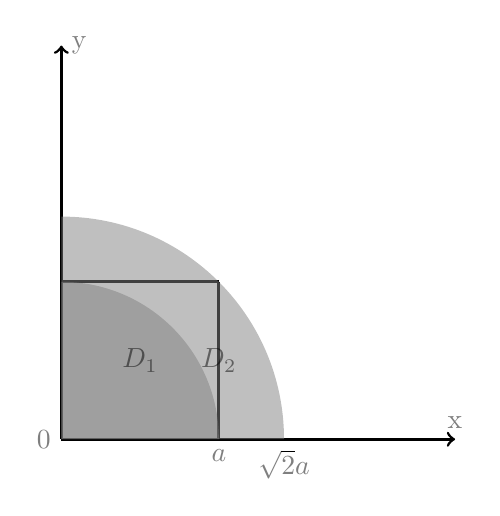
\begin{tikzpicture}[domain=1:5,line width=1pt,fill opacity=0.5]

\draw[->]  (0,0)--(5,0);
\draw[->]  (0,0)--(0,5);

\draw[-]  (2,0)--(2,2);
\draw[-]  (0,2)--(2,2);

\path [fill=gray] (0,0)-- (2,0)  arc  (0:90:2);
\path [fill=gray] (0,0)-- (2.828,0)  arc  (0:90:2.828);

\node [left] at (0,0) {0};
\node [above] at (5,0) {x};
\node [right] at (0,5) {y};

\node [below] at (2,0) {$a$};
\node [below] at (2.828,0) {$\sqrt{2} a$};
\node at (1,1) {$D_1$};
\node at (2,1) {$D_2$};

\end{tikzpicture}

$化为极坐标,\iint_{D_1} \le \iint_D \le \iint_{D_2}$

$\atinf \iint_{D_1}= \frac{\pi}{4} = \atinf \iint_{D_2},故I= \frac{\sqrt \pi}{2}(利用二重积分求\jf{0}{+\infty}e^{-x^2}dx)$

$\nl$

$截面法 \jf{e}{f}dz \iint_{S(z)}f(x,y,z)dxdy(截面规则)$

$计算Dirichlet积分 \iiint_V x^py^qz^v(1-x-y-z)^sdV(p,q,v,s \in N)$

$其中V:x+y+z=1, x=z=y=0$

$预备命题:在变换x+y=\zeta,y=\zeta \eta,下,三角形区域D:0 \le x \le 1, 0 \le y < 1-x,变为正方形D':0 \le \zeta \le 1, 0 \le \eta \le 1$

$\forall (x_1,y_1) \in D,则0 \le \zeta_1 = x_1+y_1 \le 1$

$0 \le \eta_1 = \frac{y_1}{\eta_1}= \frac{y_1}{x_1+y_1} \le 1 故(\zeta_1,\eta_1) \in D'$

$反之,\forall(\zeta,\eta)\in D',有对应(x,y)\in D$

$推广,在变换x+y+z=\zeta, y+z=\zeta \eta,z=\zeta \eta \varsigma$

$下,四面体0 \le x \le 1,0 \le y \le 1, 0 \le z \le 1, 0 \le x+y+z \le 1$

$变为正方体V',0 \le \zeta \le 1, 0 \le \eta \le 1, 0 \le \varsigma \le 1,证毕$

$现有|J|=|\frac{\partial(x,y,z)}{\partial(\zeta,\eta,\varsigma)}|=\zeta^2 \eta$

$于是有I=\jf{0}{1}\zeta^{p+q+r}(1-\zeta)^sd\zeta \jf{0}{1}\eta^{q+r}(1-\eta)^pd\eta\jf{0}{1}\varsigma^r(1-\varsigma)^q\zeta^2\eta \d\varsigma$

$=\jf{0}{1}\zeta^{p+q}(1-\zeta)^sd\zeta \jf{0}{1} \eta^{p+q-1}(1-\eta)^pd\eta \jf{0}{1}\varsigma^r (1-\varsigma)^qd\varsigma$

$=\frac{p!q!r!s!}{(p+q+r+s+3)!}$

$\jf{0}{1}dx\jf{0}{x}dy\jf{0}{xy}...dz=先xy,后xz,再yz$

$\nl$

$定理1,见P301,定理2,P302 \& P303,真正定理推广见P305 P306$

$n重积分,亦可变量替换$

$求n维单纯形T_n:x_1 \ge 0, x_2 \ge 0,...x_n \ge 0, x_1+x_2+...x_n \le a$

$\jf{n}{}dx_n=\frac{a^n}{n!}递推法$

$用归纳法证\jf{0}{t}dt_1 \jf{0}{t_1}dt_2.... =\frac{1}{n!}(\jf{0}{t}f(t)dt)^u$

$=\jf{0}{t}f(t_1)\frac{1}{(n-1)!}[\jf{0}{t}f(t)dt]^{n-1}dt_1$

$令F(x)=\jf{0}{x}f(t)dt,F'(x)=f(x)$

$=\frac{1}{(n-1)!}\jf{0}{1}F(t_1)^{n-1}f(t_1)dt_1$

$=\frac{1}{(n-1)!}\jf{0}{t}F(t_1)^{n-1}dF(t_1)$

$=\frac{1}{n!}F(t)^n$

$\nl$

$V_n=x_1^2+..x_n^2 \le R^2 体积为$

$V=\begin{cases} \frac{R^{2m}}{m!}\pi ^ m,n=2m \\ \frac{2R^{2m+1}(2\pi)^m}{(2m+1)!!},n=2m+1\end{cases}$

$\nl$

$计算\jf{0}{}x^2d\zeta 其中\zeta 为x^2+y^2+z^2=a^2,x+y+z=0交线$

$由对称性 \jf{c}{}x^2 d\zeta=\frac{1}{3}\jf{c}{}(x^2+y^2+z^2)d\zeta=\frac{a^2}{3}\jf{c}{}d\zeta=\frac{2}{3}\pi a^3$

$\nl$

$单位质点M沿着半圆从A(1,2)到B(3,4) 力\overrightarrow{F}的大小是M到原点距离$

$方向垂直于OM,且与y轴夹角小于 \frac{\pi}{2},求做功$

$分析:W=\jf{\overline{AB}}{} \overrightarrow{F} d \overrightarrow{S},|\overrightarrow{F}|=\sqrt{x^2+y^2}$

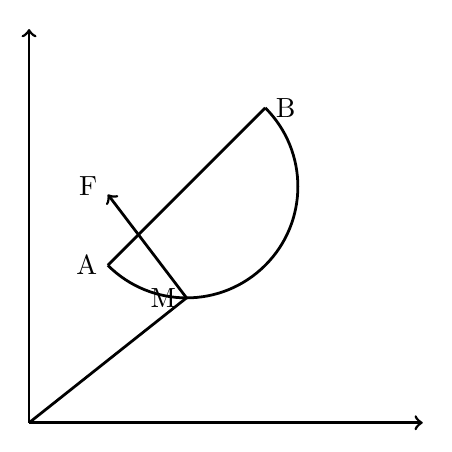
\begin{tikzpicture}[domain=1:5,line width=1pt]
\draw[->]  (0,0)  --  (0,5);
\draw[->]  (0,0)  --  (5,0);
\draw  (1,2)  --  (3,4);
\draw  (0,0)  --  (2,1.586);
\draw[->] (2,1.586)  --  (1,2.9);

\draw (1,2) arc (225:405:1.414);

\node [left] at (1,3) {F};
\node [left] at (2,1.586) {M};
\node [left] at (1,2) {A};
\node [right] at (3,4) {B};

\end{tikzpicture}

$F_x=-|\overrightarrow{F}|sin\theta,F_y=|\overrightarrow{F}|cos\theta=x$

$圆弧\overset{\frown} {AB} 记为x=2+\sqrt 2 cost,y=3+\sqrt 2 sint, t \in(-\frac{3}{4}\pi,\frac{\pi}{4})$

$W=\jf{\overset{\frown} {AB}}{} -ydx+xdy=...2(\pi-1)$

$\nl$

$定理P322,S=\frac{1}{2} \oint xdy-ydx$

$计算I=\oint_c [xcos(n,x)+ycos(n,y)]ds,\overrightarrow n为c的外法线方向$

$解:(n,x)=(\tau,y);(u,y)=\pi - (\tau,x)$

$cos(u,x)ds=cos(\tau,y)ds=dy$

$cos(n,y)ds=-cos(\tau,x)ds=-dx$

$I=\oint_cxdy-ydx=2S_{面积}$

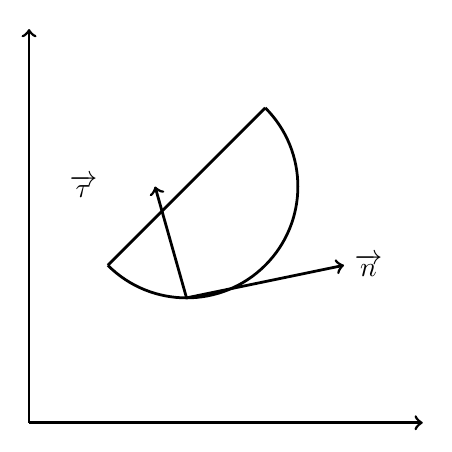
\begin{tikzpicture}[domain=1:5,line width=1pt]
\draw[->]  (0,0)  --  (0,5);
\draw[->]  (0,0)  --  (5,0);
\draw  (1,2)  --  (3,4);
\draw[->]  (2,1.586)  --  (4,2);
\draw[->] (2,1.586)  --  (1.6,3);

\draw (1,2) arc (225:405:1.414);

\node [left] at (1,3) {$\overrightarrow \tau$};
\node [right] at (4,2) {$\overrightarrow n$};

\end{tikzpicture}

$C为闭曲线,\overrightarrow l 为给定的方向,则有\oint_c cos(l,n)ds=0$

$\overrightarrow n 为c的外法线方向$

$分析:(l,n)=(l,x)-(n,x)$

$cos(l,n)=cos(l,x)cos(n,x)+sin(l,x)sin(n,x)$

$sin(n,x)=sin((\tau,x)-\frac{\pi}{2})=-cos(\tau,x)$

$cos(n,x)=cos((\tau,x)-\frac{\pi}{2})=sin(\tau,x)$

$cos(\tau,x)ds=dx$

$sin(\tau,x)ds=dy$

$\oint_c cos(l,n)ds= cos(l,x)dy-sin(l,x)dx$

$\oint_c -sin(l,x)dx=sin(l,x)\oint_c dx=0$

$\oint_c cos(l,x)dx=cos(l,x)=0,故有。。。。$

$\nl$

$计算I=\oint_c \frac{-ydx+xdy}{x^2+y^2},c为任一闭合曲线,取正方向$

$分析:c不含原点时,\frac{\partial P}{\partial y} = \frac{\partial Q}{\partial x}=...$

$c含原点时,作小圆c_\epsilon 取正方向,I=-\jf{c_\epsilon}{}Pdx+Qdy$

$=-\frac{1}{\epsilon^2}\jf{c_\epsilon} xdy-ydx 面积公式$

$=-\frac{1}{\epsilon^2}(2\pi \epsilon^2)$

$=2\pi$

$\nl$

$证明:\iint_D(\frac{\partial ^2f}{\partial x^2}+\frac{\partial ^2f}{\partial y^2})dxdy= \oint_c \frac{\partial f}{\partial \eta} ds,c为区域D的边界取正向,\frac{\partial f}{\partial \eta}为$

$f(x,y)在c上P(x,y)处沿外法线\overrightarrow \eta 的方向导数$

$分析:\frac{\partial f}{\partial \eta} = \frac{\partial f}{\partial x}cos(\eta,x)+\frac{\partial f}{\partial y}cos(\eta,y)$

$=\frac{\partial f}{\partial x}cos(\tau,y)-\frac{\partial f}{\partial y}cos(\tau,x)$

$\nl$

$第二型曲面积分$

$一、曲面的例$

$在光滑曲面上\sigma 上任取一点P_0(x_0,y_0,z_0)过P_0点法线\overrightarrow \eta 的方向规定如下:$

$1. 若\sigma:z=z(x,y),\eta 正方向与z轴正方向成锐角的一侧为正侧(x,y类似)$

$2.封闭曲面,外侧为正,内侧为负$

$定义1,设\overrightarrow F = (P(x,y,z)Q(x,y,z)R(x,y,z))是定义在光滑或分段光滑曲面$

$\sigma 上,取定\sigma 的一侧\overrightarrow n = (cos \alpha, cos \beta, cos \gamma),按第二型曲$

$面积分方法,对\sigma 作任意分法T和任意取法\{M_r\}若极限$

$\lim\limits_{nT \to 0} \ksum{1}{n}P(M_k)cos \alpha_k \Delta S_k$

$\lim\limits_{nT \to 0} \ksum{1}{n}Q(M_r)cos \beta_k \Delta S_k$

$\lim\limits_{nT \to 0} \ksum{1}{n}R(M_k)cos \gamma_k \Delta S_k 都存在,则定义$

$\iint_{\Sigma}Pdydz+Qdzdx+Rdxdy=\iint_(Pcos\alpha+Qcos\beta+Rcos\gamma)ds$

$=\iint_{\Sigma} \overrightarrow F \overrightarrow n ds$

$\nl$

$定理1,设R(x,y,z)是光滑或者分段光滑曲面\Sigma,z=z(x,y)$

$(x,y)\in P_{xy}上的连续函数,则R在\Sigma 上对xy第二型曲面积分$

$\iint_{\Sigma}R(x,y,z)dxdy=\pm \iint_{D(x,y)}R(x,y,z(x,y))dxdy$

$其中\pm 对应曲面的侧$

$注:若曲面\Sigma 与平行于z轴的直线交于两点,则应分\Sigma 为\Sigma_1 \Sigma_2$

$\Sigma_1: z=z_1(x,y)...(x,y) \in D_1$

$\Sigma_2: z=z_2(x,y)...(x,y) \in D_2$

$且\iint_{\Sigma}R(x,y,z)dxdy=\iint_{D_1}R(x,y,z_1)dxdy-\iint_{D_2}R(x,y,z_2)dxdy(见P325)$

$\nl$

$复合函数二阶偏导数$

$函数可微性(\lim \frac{\Delta z-dz}{p}=0)$

$二元函数极限,累次$

$方向导数$

$隐函数(组)求导(空间切线,切面)$

$方程变换(自变量与公式变换)$

$多元函数极值$

$含参数积分一致收敛,计算(求导,换序)可导性,连续性$

$重积分(不含n重)(极坐标,柱坐标,球坐标)$

$应用(质心,质量引力矩)$

$曲线曲面积分$

$场:梯度,旋度,散度,三场$

$定理:(P151,换序定理)(P206 隐函数存在)(P225 连续定理)$

$(P335格林公式)(P349平面曲线,4个循环)$

$\nl$

$散度div \overrightarrow F(M)= \vtx{M} \frac{1}{v} \iint_{\Sigma} \overrightarrow F \overrightarrow n ds= \triangledown \overrightarrow F$

$ \iint_{\Sigma} \overrightarrow F \overrightarrow n ds =\iiint_v \triangledown \overrightarrow F dxdydz$

$div(\overrightarrow F+\overrightarrow G)= div\overrightarrow F + div\overrightarrow G$

$div(n \overrightarrow c)= \overrightarrow c grad u$

$div(u \overrightarrow F)= udiv \overrightarrow F +\overrightarrow F grad u$

$V(u \overrightarrow F)=u \triangledown \overrightarrow F+\overrightarrow F \triangledown u$

$\nl$

$例:div(grad u)= div(\frac{\partial u}{\partial x} \overrightarrow i+\frac{\partial u}{\partial y} \overrightarrow j+ \frac{\partial u}{\partial z} \overrightarrow k)$

$=\frac{\partial ^2 u}{\partial x^2} + \frac{\partial ^2 u}{\partial y^2} + \frac{\partial ^2 u}{\partial z^2} \triangleq \Delta u$

$div(u grad u)=udiv(grad u)+grandu grandu$

$=u\Delta u+\triangledown u \triangledown u$

$\nl$

$求\overrightarrow u = yz \overrightarrow i + zx \overrightarrow j + xy \overrightarrow k的流量$

$(1)穿过圆柱x^2+y^2=a^2的侧表面(0 \le z \le h)$

$Q=\iint_yzdydy+zxdxdz+xydxdy$

$(3)加上上底下底流量$

$Q=\iint (\frac{\partial yz}{\partial x}+\frac{\partial zx}{\partial y}+\frac{\partial xy}{\partial z})dxdydz=0$

$\nl$

$例:已知\overrightarrow A,求u(x,y,z)使得\overrightarrow A 成为u梯度,称u为势函数,u含常数c$

$\nl$

$有势场,设\overrightarrow A(M),M \in V 为向量场,称\overrightarrow A 为有势场,存在u,\forall (x,y,z) \in V 有$

$grad \bold u=\overrightarrow A(P369)$

$设\overrightarrow A(m)为向量场:m \in V,\forall M \in V,div \overrightarrow A =0(无源场)$

$则\overrightarrow A 为管状场$

$调和场:rot \overrightarrow A =\overrightarrow 0, div \overrightarrow A = 0(无旋无源)$

$调和场\overrightarrow A 必有势函数,且满足Laplace方程:\frac{\partial ^2u}{\partial x^2} + \frac{\partial ^2u}{\partial y^2} + \frac{\partial ^2u}{\partial z^2} = 0$
\end{document}

